
\todo[inline]{change figure caption to general S matrix notation}
\begin{figure}[h]
\centering
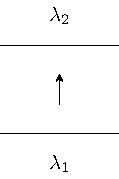
\includegraphics{fig_lambda_1_lambda_2.pdf}
\caption{Partition function between two boundary states $\lambda_1$ and $\lambda_2$}
\label{fig:fig_lambda_1_lambda_2}
\end{figure}

In this appendix, we calculate the amplitude between general boundary states (\cf  Eq.~\eqref{eq:bd_state})
\begin{equation}
\exp\Big\{  \vec{b}^{\dagger} S_a( \theta )   \vec{\bar{b}}^{\dagger}\Big\}  |0  \rangle
\end{equation}
where we have used the vector notations for the set of Bosons. The $S$ matrices therein can be any one of the two types in Eq.~\eqref{eq:S1_S2}. 

Let the cylinder has height $2\pi$ and width $\beta \gg 1 $, the partition function between the two boundary states is
\begin{equation}
Z_{ab} =  \langle a | e^{ - 2\pi H } |b \rangle 
\end{equation}
where the Hamiltonian
\begin{equation}
H = \frac{2\pi}{\beta} (L_0 + \bar{L}_0) =  \frac{4\pi}{\beta}  L_0 = \frac{4\pi}{\beta}\sum_{n > 0 }  n b_n^{\dagger} b_n. 
\end{equation}
In this expression, we have neglected the $-\frac{c}{24}$ term for it has been considered in App.~\ref{app:F_correction}. We have also used the boundary state condition $L_n = \bar{L}_n$ valid for the boundary state. The partition function then becomes
\begin{equation}
Z_{ab} = \langle 0 | \exp\Big\{ \vec{b} S_a^* \vec{\bar{b}}\Big\} \exp\Big\{ - \vec{b}^{\dagger} \mathbb{I}_2 \otimes M  \vec{b} \Big\}   \exp\Big\{  \vec{b}^{\dagger} S_b  \vec{\bar{b}}^{\dagger}\Big\}  |0  \rangle  = \frac{1}{\det ( 1 - S^{\dagger} _a  e^{- \mathbb{I}_2 \otimes M} S_b) }
\end{equation}
where
\begin{equation}
M =  \frac{4\pi^2}{\beta} \text{diag}( 1, 2, \cdots ) \quad  \mathbb{I}_2 = \text{diag}( 1, 1) 
\end{equation}
Using the fact that their determinants are $|\det( S_a S_b^{\dagger})|  = 1$, we have the free energy 
\begin{equation}
F = - \ln |Z_{ab}| = \ln |\det ( S_a S_b^{\dagger} - e^{- \mathbb{I}_2 \otimes M} )|
\end{equation}
There are two cases to be considered, and we only take out the leading order term in $\beta$. 
\begin{itemize}
\item {\it case 1: }$S_1( \theta_1 ) \rightarrow S_2 ( \theta_2 ) $, the free energy is
\begin{equation}
\begin{aligned}
F & = \ln |\det ( S_1( \theta_1 )  S_2^{\dagger}( \theta_2 )  - e^{- \mathbb{I}_2 \otimes M} )| \\
  & = \ln \left| \det
\begin{bmatrix}
-\cos 2 \Delta \theta \mathbb{I} - e^{-M}   & -\sin 2 \Delta \theta \mathbb{I}\\
- \sin 2\Delta \theta \mathbb{I}  &   \cos 2 \Delta \theta \mathbb{I} - e^{-M} \\ 
\end{bmatrix} \right| \\
& = \sum_i \ln [ 1 -  e^{- 2 \lambda_i }  ] = \frac{\beta}{4\pi^2} \int_0^{\infty} dx \ln [ 1 - e^{-2x} ]  = - \frac{1}{48 }\beta 
\end{aligned}
\end{equation}
\item {\it case 2:} $S_i( \theta_1 ) \rightarrow S_i( \theta_2 )$, where $i = 1 $ or $ 2$, 
\begin{equation}
\begin{aligned}
F & = \ln \det 
\begin{bmatrix}
\cos 2 \Delta \theta \mathbb{I} - e^{-M}   & \sin 2 \Delta \theta \mathbb{I}\\
- \sin 2\Delta \theta \mathbb{I}  &   \cos 2 \Delta \theta \mathbb{I} - e^{-M} \\ 
\end{bmatrix} \\
& = \sum_i \ln [ 1 - 2 \cos 2 \Delta \theta e^{- \lambda_i } + e^{- 2 \lambda_i }  ] \\
& = \frac{\beta}{4\pi^2} \int_0^{\infty} dx \ln [ 1 - 2 \cos 2 \Delta \theta e^{-x} + e^{-2x} ] 
\end{aligned}
\end{equation}
where $\Delta \theta = \theta_2 - \theta_1$. This integral is an even function of $\Delta \theta$ and the $\Delta \theta > 0$ case reduce to the polylog and Bernoulli polynomial
\begin{equation}
\begin{aligned}
  F &= \frac{\beta}{4\pi^2} \left[ - \text{Li}_2 ( e^{2i |\Delta \theta|} ) - \text{Li}_2 ( e^{- 2i |\Delta \theta|} ) \right] \\
  & = \frac{\beta}{4\pi^2}  \left[ - 2\pi^2 B_2 (x) \right] \\
  &= - \frac{\beta}{2} B_2( |x| )  = \frac{\beta}{2} (| x| - x^2 - \frac{2}{6} )
\end{aligned}
\end{equation}
where $x = \frac{\Delta \theta}{ \pi}$. 
\end{itemize}




%%% Local Variables:
%%% TeX-master: "bCFT_paper"
%%% TeX-PDF-mode: t
%%% End:
